\section{Results and discussion}\label{sec:result}
We will now first take a look at the case of two electrons in a potential with different oscillator energies. In order to do so, we perform a Variational Monte Carlo simulation and use the Metropolis algorithm explained in section~\ref{sec:metropolis} to find the energy of the ground state. Therefor we use numerical derivation. We will later introduce analytical calculations based on closed-form expressions as well (section~\ref{sec:analytical}). Besides, we put emphasis on the correlations introduced by the Jastrow factor by computing the kinetic and potential energy of the ground state for different oscillator frequencies.\\
In addition we introduce importance sampling and analyse the dependency of the results to the time step $\delta t$.\\
\subsection{Two electron case}\label{sec:2electron}
Since it is the easiest case, we first look at two electrons in a quantum dot interacting with each other. According to \cite{lohne2011} the corresponding energy is at $E = 3~\mathrm{a.u.}$ (atomic units).\\
For the computation we use the variational wave function
\begin{equation}
\psi_T(\mathbf{r_1,r_2}) = C \exp\left[-\alpha\frac{\omega}{2} (r_1^2+r_2^2)\right] \exp \left[ \frac{a_{12} r_{12}}{(1+\beta r_{12})} \right],
\end{equation}
where we start by considering a wide range of $\alpha \in[0.7,1.3]$ and $\beta \in[0.2,0.6]$ first and perform a more precise simulation afterwards. The goal is to find the variational parameters $\alpha$ and $\beta$, where the energy is at its minimum. After the first simulation we notice, that the minimum must be somewhere around $\alpha \in[0.9,1.1]$ and $\beta \in[0.35,0.45]$. This is why we preform a simulation with these boundaries and use 3 000 000 Metropolis cycles to get an accurate result. In figure~\ref{fig:2electron} the energy is plotted depending on both variational parameters $\alpha$ and $\beta$. The 3D-plot results in a bended plane resembling to the shape of a valley. For increasing $\alpha$ the corresponding $\beta$ at minimal energy is decreasing. The minimum energy calculated is 
\begin{align}
E &= 3.0003~\mathrm{a.u.}
\intertext{at}
\alpha &= 0.9867,\\
\beta &= 0.4033.
\end{align}
As mentioned before we were expecting the energy to be at $E=3~\mathrm{a.u.}$, so the calculated value matches the expected one very well. In figure~\ref{fig:2electron} there are some areas, where the plane is not as smooth as in others. We classify these small perturbations to the valley as numerical fluctuations and consider them to be stronly important.\\
To get a better understanding of the influence the parameters have on the calculated energy, figure~\ref{fig:2electronalpha} shows the energy's $\alpha$-dependency for different $\beta$. Consistent with figure~\ref{fig:2electron} this figure reveals, that $\beta$ is shifted depending on $\alpha$ and that $\alpha$ has a larger influence on the energy than the other variational parameter. The errors plotted in figure~\ref{fig:2electronalpha} are almost invisible, since they are very small compared to the energy fluctuations at varying $\alpha$ and $\beta$. There are not many cases, where the error is significantly high, so we consider our results to be of sufficient accuracy.
\begin{figure}[htbp]
    \centering
    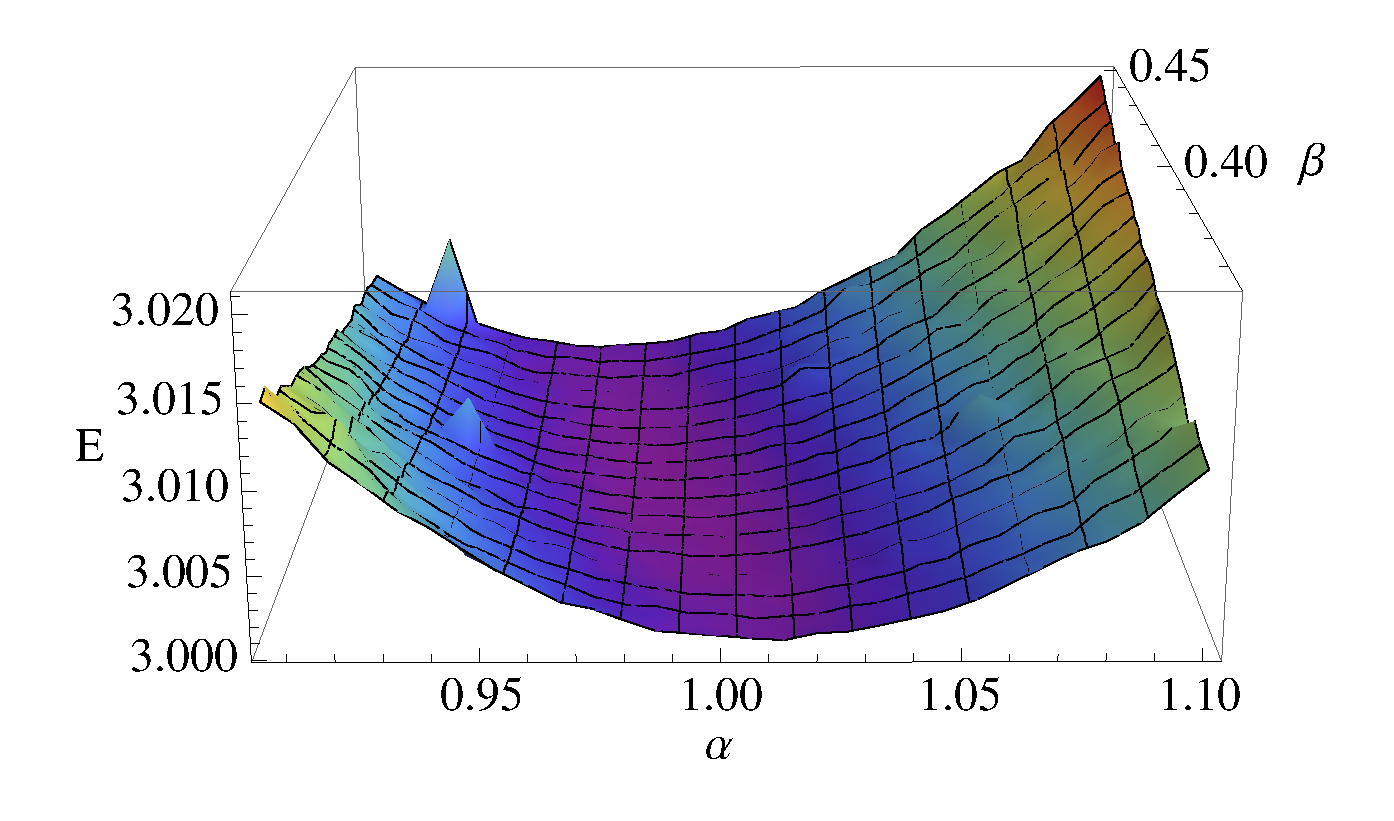
\includegraphics[scale=0.6]{2electron}
    \caption{Plot of $\alpha$- and $\beta$-dependencies of the ground state energy for two interacting electrons at the ground state based on a simulation involving 3 000 000 Metropolis cycles}
    \label{fig:2electron}
\end{figure}
\begin{figure}[htbp]
    \centering
    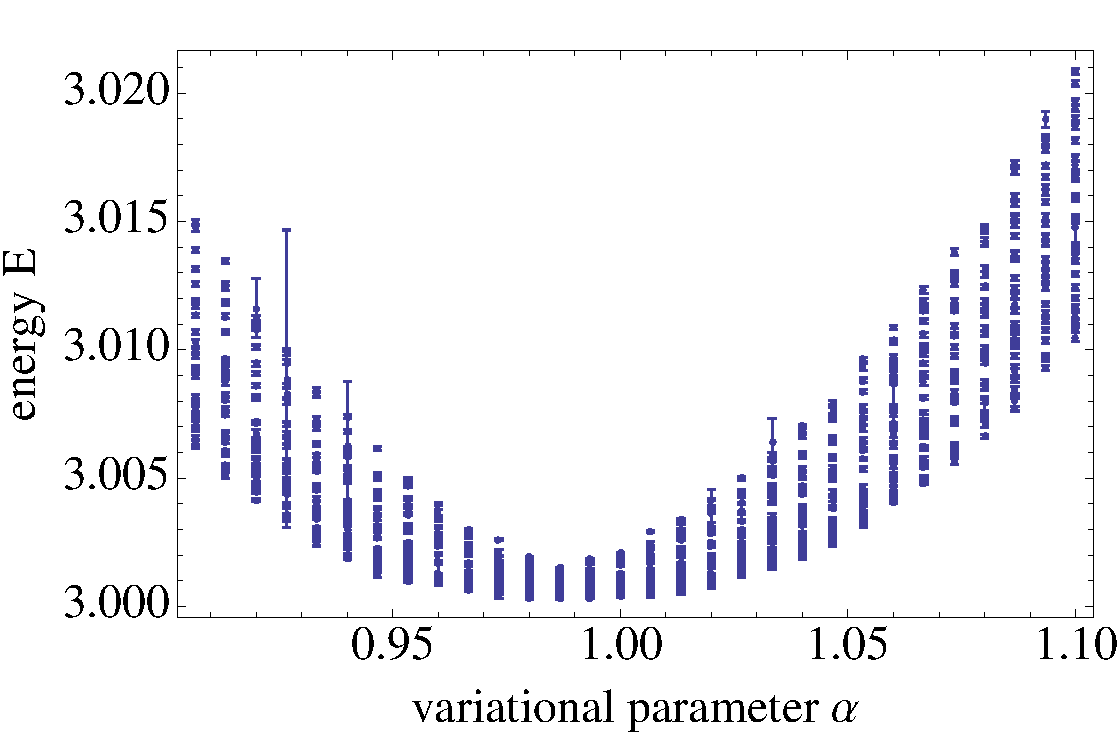
\includegraphics[scale=0.6]{2electronalpha}
    \caption{Plot of $\alpha$-dependency of the ground state energy for two interacting electrons at the ground state for different $\beta$ based on a simulation involving 3 000 000 Metropolis cycles}
    \label{fig:2electronalpha}
\end{figure}
\FloatBarrier
\subsubsection{Jastrow factor}
After computing the ground state energy we now analyse the changement in energy arising from different osciallator potentials $\omega$. The results for $\omega =\{1,0.28,0.01\}$ are shown in table~\ref{tab:omega}. It can be observed, that for small oscillator frequency the kinetic energy drops relative to the total energy of the system. The reason for this is, that for small $\omega$ the potential gets wider, but flatter as well. In this case, the electrons interact less with each other, which results in decreasing kinetic energy.\\
\begin{table}[H]
\centering
\caption{Kinetic and potential energy depending on the oscillator frequency $\omega$}
\begin{tabular}{c|cc|cc}
$\omega$ & $E_{kin} \mathrm{(a.u.)} $& $E_{pot} \mathrm{(a.u.)}$ & $E_{kin}/E \mathrm{(\%)}$ & $E_{pot}/E \mathrm{(\%)}$ \\ \hline
1.00    & 0.8891  & 2.111  & 29.6 & 70.4 \\
0.28 & 0.2616  & 0.774  & 25.3 & 74.7 \\
0.01 & 0.0106 & 0.096 & 9.9 & 90.1
\end{tabular}
\label{tab:omega}
\end{table}
In the wave equation
\begin{equation}
\psi_T(\mathbf{r_1,r_2}) = C \exp\left[-\alpha\frac{\omega}{2} (r_1^2+r_2^2)\right] \exp \left[ \frac{a_{12} r_{12}}{(1+\beta r_{12})} \right]
\end{equation}
only the first exponential term is affected by the oscillator frequency $\omega$, while the Jastro factor does not contain the frequency.\\
For vanishing potential as for $\omega =0.01$ the wave function becomes:
\begin{equation}
\lim_{\omega\rightarrow 0} \psi_T(\mathbf{r_1,r_2}) = C \exp \left[ \frac{a_{12} r_{12}}{(1+\beta r_{12})} \right] = C J,
\end{equation}
where $J$ is the Jastrow factor. This means, that in this case the Jastrow factor adopts a more important role. The correlations introduced by the Jastro factor ...
\subsubsection{Importance sampling: $\delta t$-dependency}
To obtain accurate results we also introduce important sampling and optimize the calculation of the energy by studying its time step dependency. We will refer to the time step as $\delta t$. The time step plays an important role in importance sampling, since it the biasing when calculation new random numbers. For large $\delta t$ the newly picked random numbers for the particle position can vary more, than for smaller $\delta t$. It is therefore relevant to use a reasonable time step to aviod jumping to far in the position or to get stuck in one place as explained previously in section~\ref{sec:importance}. In figure~\ref{fig:importance} we plotted the energy calculated for $\alpha = 0.98$ and $\beta = 0.40$ (according to~\ref{sec:2electron}) for diverse $\delta t$. Comparing the results including importance sampling to those in section~\ref{sec:2electron} we notice, that with importance sampling we can obtain a lot smaller energies, than when using a brute force Metropolis algorithm. This shows, that the importance sampling has an impact on the precision of the results, because we get energies very near the exact solution.\\
Concerning the optimal value of $\delta t$, it is obvious in figure~\ref{fig:importance}, that it must be $\delta t \in [0.1,0.2]$. Because of the statistical spread of the energy values, we cannot find the one and only perfect $\delta t$-value. For large time steps the energy converges to $E=3.0016$ ...
%Gleicher Wert wie in Aufgabenteil b)?
\begin{figure}[htbp]
    \centering
    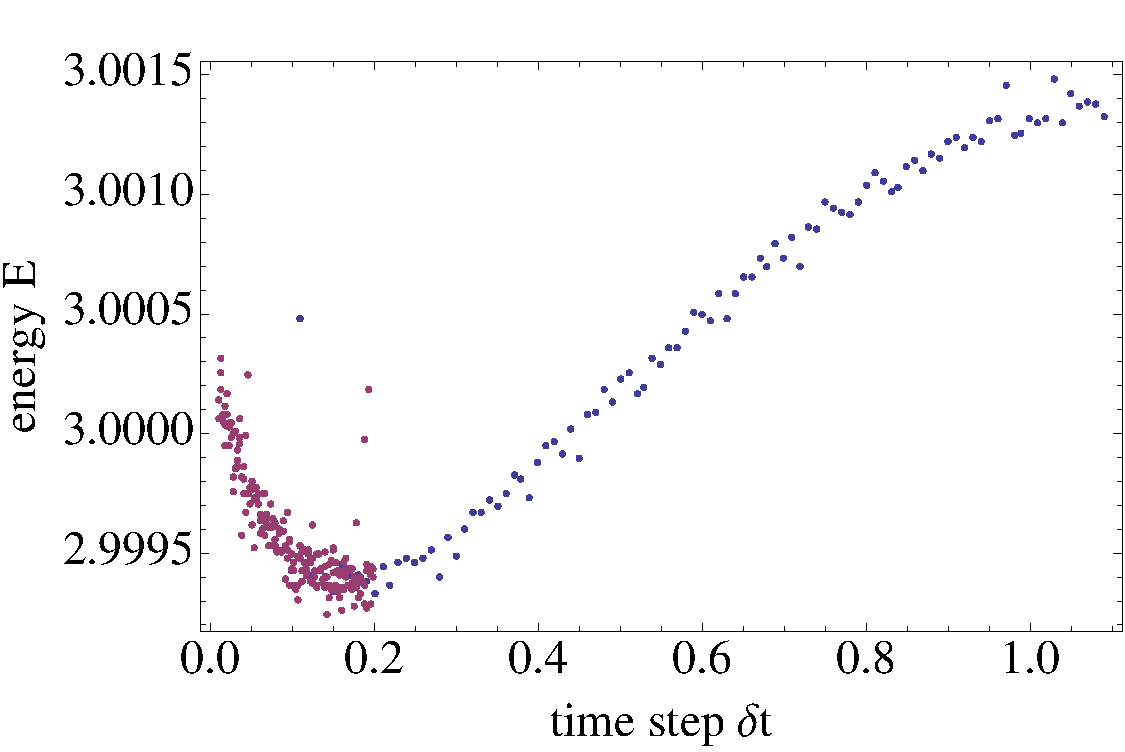
\includegraphics[scale=0.6]{importance}
    \caption{Results of energy calculation for varying time steps $\delta t$ in the importance sampling. The blue dots refer to a wide-spaced simulation for $\delta t \in [0.1,1]$ with step length $\Delta (\delta t) = 0.01$, whereas the violet dots refer to $\delta t\in [0.01,0.2]$ with $\Delta(\delta t) = 0.001$}
    \label{fig:importance}
\end{figure}
\FloatBarrier

\subsection{Six electron case}
In this part we introduce the six electron case. In order to do so we consider the more general trial wave function \ref{glg:6electron} which also includes the case of two electrons. The simulations are done like in section \ref{sec:2electron} but with $400000$ cycles, because of higher computation times.

\subsubsection{Perturbed Case}\label{sec:perturbed_six}
For the perturbed six electron system the ground state energies are shown in table \ref{tab:groundstate_sixelectron}. Comparing the energies with \citet[TABLE III]{lohne2011} we have a good agreement but slightly larger values. For increasing $\omega$ we have higher values of $\alpha$ and $\beta$. Figure \ref{fig:alpha_beta_omega} shows the dependencies in this case. It can be seen that there is no easy linear coherence, instead we made an arbitrarily chosen fit with a square-root function which seemed for us the best approximation and deals a reference where to search for the energy minima for different $\omega$. 
\begin{table}
    \centering
    \caption{Ground state energies for six electrons in an oscillator well.}
    \begin{tabular}{c|cc|c}
    $\omega$   & $\alpha$    & $\beta$ &    $E$    \\ \hline
    $1.00$     & $0.98$      & $0.45$  & $20.185$  \\
    $0.5$      & $0.925$	    & $0.38$  & $11.8047$ \\
    $0.28$     & $0.8$       & $0.25$  & $7.736$   \\
    $0.01$     & $0.7$       & $0.08$  & $0.6986$  \\
    \end{tabular}
    \label{tab:groundstate_sixelectron}
\end{table}
\begin{figure}[htbp]
    \centering
    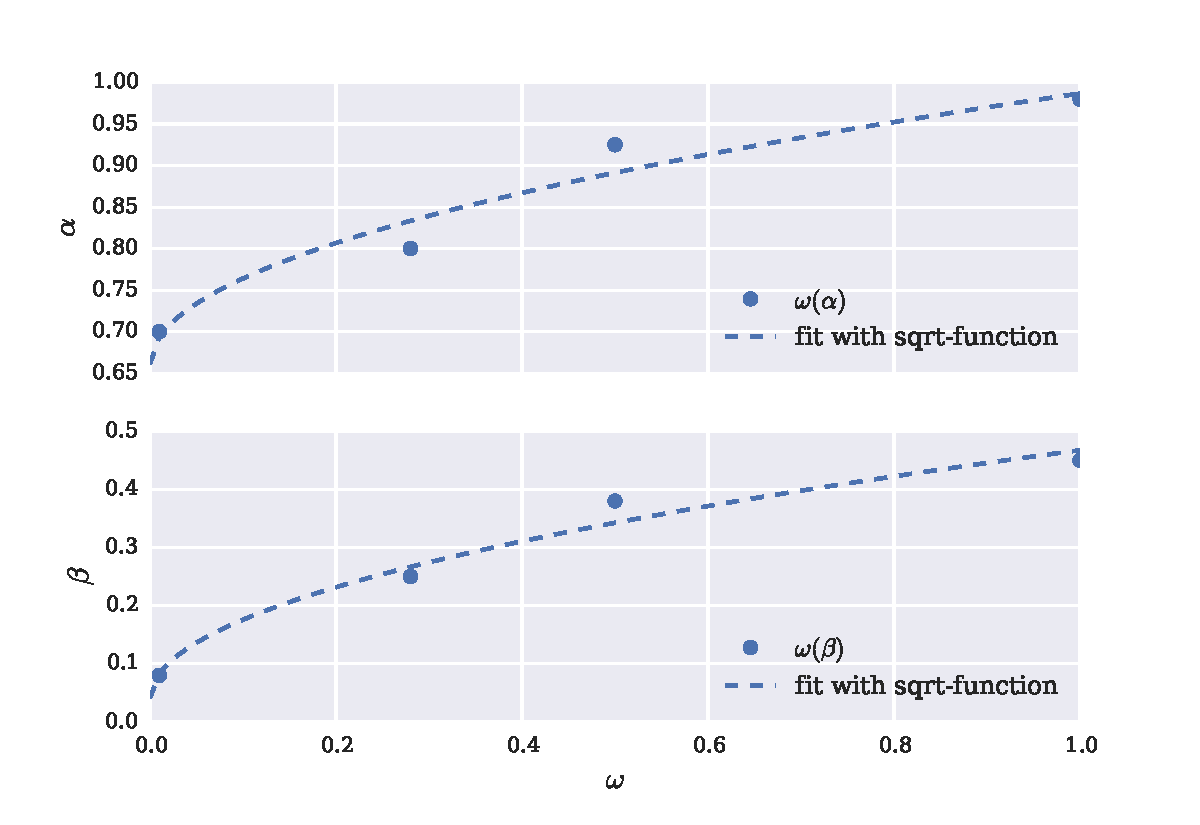
\includegraphics[scale=0.7]{alpha_beta_omega.pdf}
    \caption{Shows the dependency between the locations of the energy minima and the variational parameter.}
    \label{fig:alpha_beta_omega}
\end{figure}

All in all our code seems to calculate reliable and good energies. Nevertheless we had to struggle with rather seldom but randomly appearing negative kinetic energies in single cores when using importance sampling. Changing our initial guesses for the starting positions increased here the quality of the solution considerably. In Appendix \todo{reference} are shown some three-dimensional plots which show the problem. 

\subsubsection{Unperturbed Case}
We know that with switched off electron-electron repulsion the lowest energy value should become $10\,\omega$, since we are observing six electrons. In figure \ref{fig:six_electron_unperturbed} this relation is shown for different $\omega$ over $\alpha$ and it can be observed that our results fit very well to the theory. 
\begin{figure}[htbp]
    \centering
    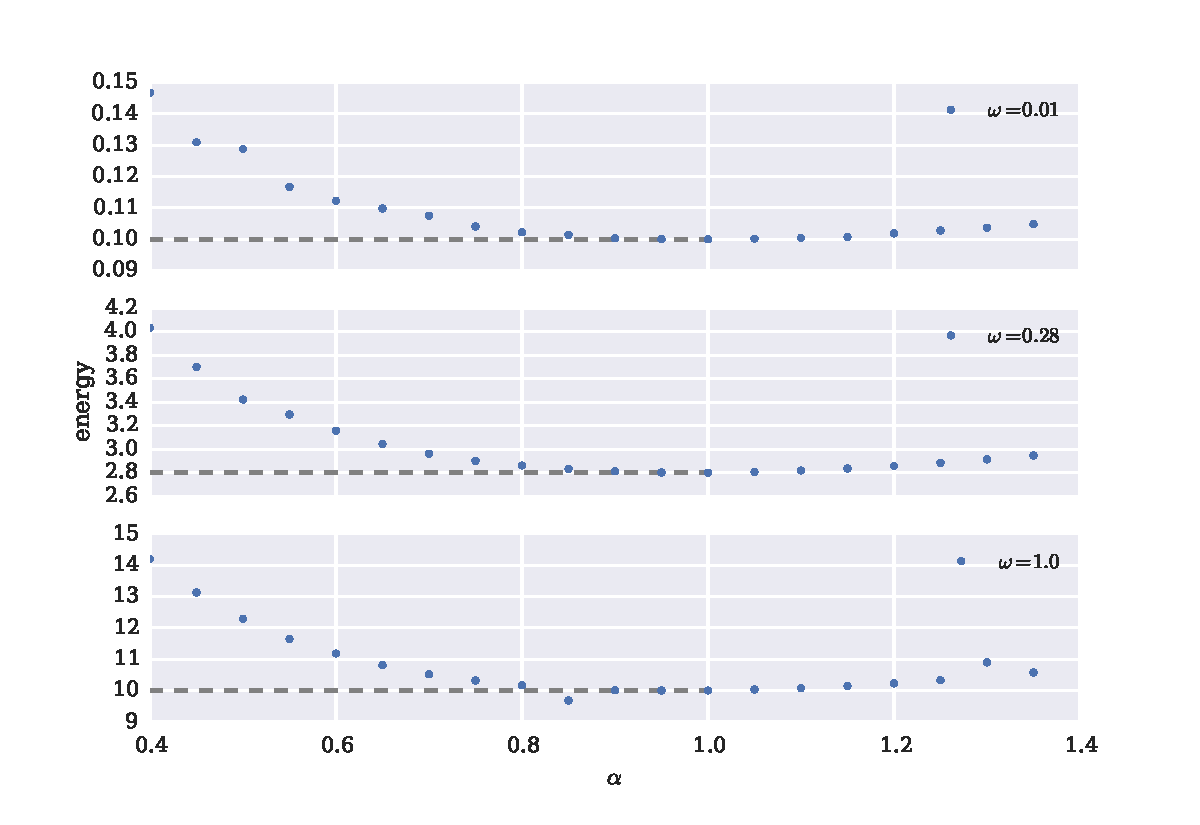
\includegraphics[scale=0.7]{six_electron_unperturbed}
    \caption{The figure shows the energy plotted over the variational parameter $alpha$ assuming six electrons without the repulsive electron-electron forces. For different values of $\omega$ the minimum lies at $10\omega$ which is coherent with the theoretical view.}
    \label{fig:six_electron_unperturbed}
\end{figure}

\subsubsection{Virial theorem}
The virial theorem states a relationship between the mean of the potential $\langle V \rangle$ and of the kinetic energy $\langle T \rangle$ of a closed system. This is described by
\begin{equation}
    \gamma \langle V \rangle = 2 \langle T \rangle,
\end{equation}
with $\gamma$ the homogeneity of the potential $V$. This means for a harmonic oscillator which potential goes with the power of $2$ that one can expect the relationship $\langle V \rangle = \langle T \rangle$. However if we consider the perturbed wavefunction we have additional terms which are stated by the repulsion of the electron and would reveal $\gamma = -1$. Hence, we can make the prediction that the perturbed wavefunction should yield to a smaller ratio 
\begin{equation}
\left(\frac{\langle V \rangle}{\langle T \rangle}\right)_{perturbed} \leq \left(\frac{\langle V \rangle}{\langle T \rangle}\right)_{unperturbed},
\end{equation}
whereas the difference should be larger for smaller $\omega$, because thereby the oscillator potential becomes less relevant. Meanwhile for different $\omega$ and the unperturbed case the ratio should not change and be unity.

In figure \ref{fig:virialtheorem} this behaviour is shown and mostly consistent. Considering first the two electron case we can observe for the unperturbed wavefunction a ratio that is nearly one for all omega. The perturbed part indeed shows the predicted behaviour that it is firstly smaller and secondly it increases with increasing omega. For the six electron system the perturbed functions have the same dependencies as for two electrons with even smaller ratios. This can be physically understood as a more important role for the electron-electron interactions in the six electron case which go with $\gamma = -1$. For the unperturbed part there is a small deviation to unity for larger omegas. This shouldn't be the case and reveals a potential problem in the code for multiple particles. Indeed the data shows that there might be an issue in the draft of the slater matrix. However taking also in reference the known issues of section \ref{sec:perturbed_six} it could also depend on the important sampling but still after extensive search we were not able to find a malfunction and all other calculations run reasonable which leads us to the conclusion that the energies that are produced by our code are reliable values.  
\begin{figure}[htbp]
    \centering
    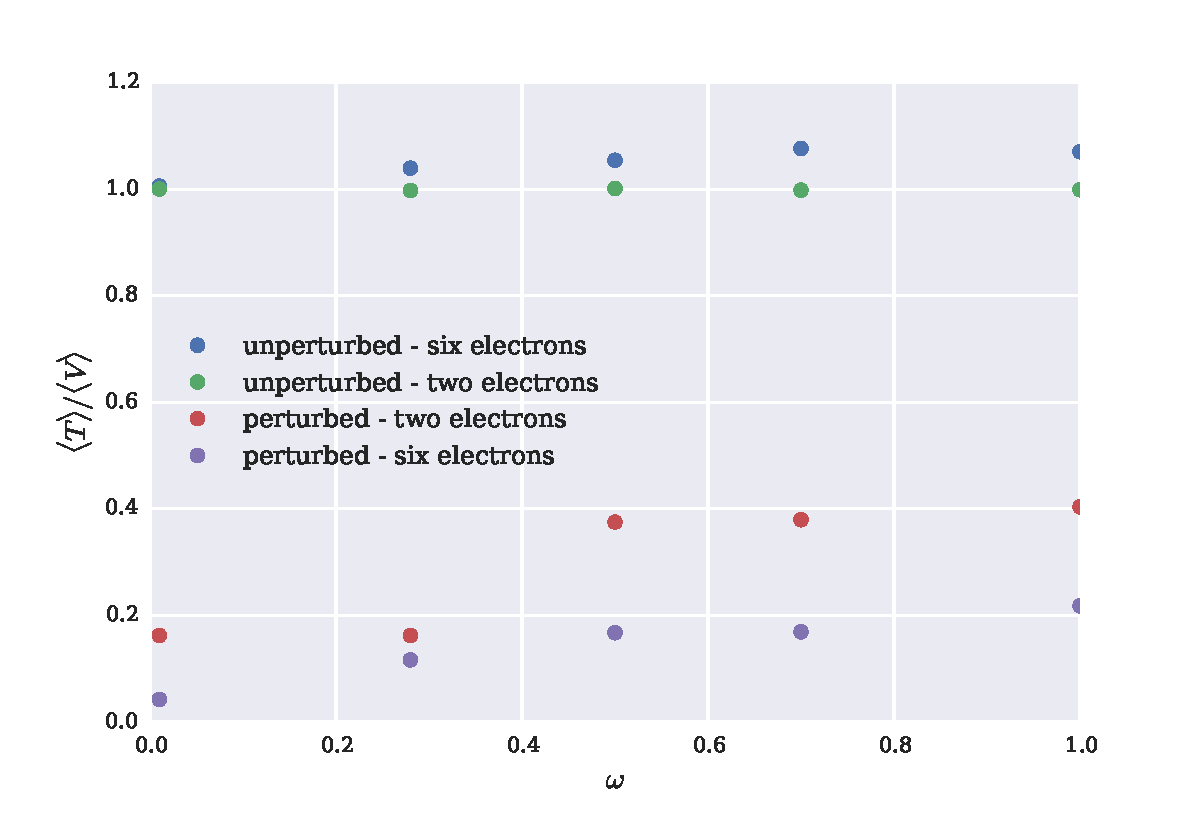
\includegraphics[scale=0.7]{virialtheorem}
    \caption{Shows the fraction of the mean kin. energy $\langle T \rangle$ to the mean pot. energy $\langle V \rangle$ for different values of $\omega$. The calculations are done with either two or six electrons. The unperturbed function}
    \label{fig:virialtheorem}
\end{figure}

\subsection{Closed form solutions}\label{sec:analytical}
Finally we still want to introduce calculations with the closed form solutions described in section \ref{sec:closed_form}. For that reason the program was restructured in parts and new classes for the Jastrow-factor and the Slater-matrix were introduced. This can be found at the separate branch \texttt{closed_form} at the provided git repository. The part is fully implemented but unfortunately we were not able to reproduce the solution of the brute force approximations. But still because we implemented the full code, we were able to calculate the profiling and can make first estimations how much faster the code could be. We thereby implemented no optimizations, like an improved calculation of the inverse slater matrix yet (see \citet{hogberget2013} for more details). An overview for the profiling is given in the table \ref{}\todo{reference}.